\chapter{Implementation, Integration and Test Plan}
\label{cha:impl}

\section*{Implementation}
Here we explain how a possible good order of implementation of subcomponents might help us to fulfill and build the application. Its achievement implies the following steps:
\begin{itemize}
\item We first plan to configure all server components (since they are those which will be queried by the client application afterwards), which, basically, ranges from creating a user pool (AWS Cognito) for data synchronization and authentication to setting up the cloud storage (AWS S3 or DynamoDB) for backing up and archiving data in order to provide the best user experience. 
\item We focus on the creation of the client application, whose order of modules (handlers) is illustrated in Figure \ref{fig:componentsDiagram}.
\end{itemize}

\begin{figure}[H]
	\centering
	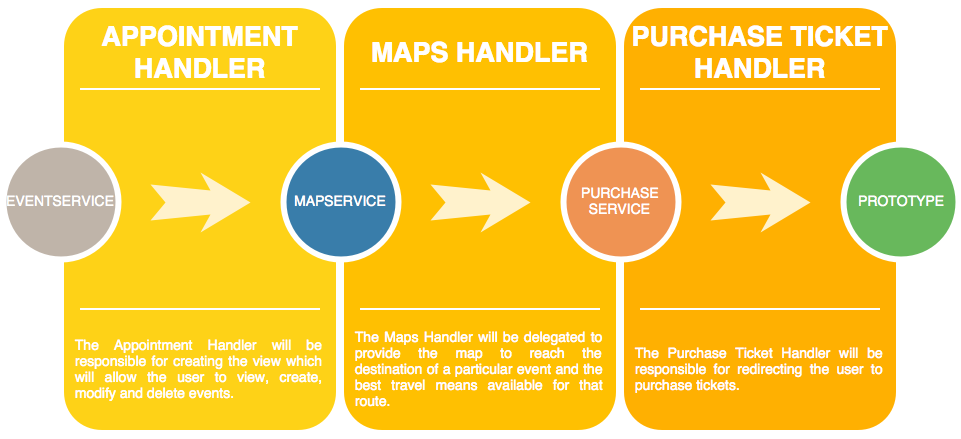
\includegraphics[width=6.5in]{./diagrams/ComponentsOrderDiagram.png}
	\caption{Order of main components of the client application to be deployed.}
	\label{fig:componentsDiagram}
\end{figure}

\section*{Integration}
Here we describe how integration strategies are supposed to be performed. Specifically, we explain how different components are integrated in our system and which strategy we adopt in order to integrate all components efficiently.

\subsection*{Elements to be integrated}
\label{sub:delemenetsIntegrated}
The following list represent every component grouped into several subsystems: \newline

\textbf{Core Data}
\begin{itemize}
\item AWS Cognito Sync
\item AWS Data Manager
\item AWS S3 / DynamoDB DBMS
\end{itemize}

\textbf{Account Management}
\begin{itemize}
	\item AWS Cognito for Authentication
	\item AWS Cognito for Account Management
\end{itemize}

\textbf{Event Management}
\begin{itemize}
  \item Appointment Manager
  \item Notification Manager
\end{itemize}

\textbf{Maps Management}
\begin{itemize}
	\item Google Maps API
    \item Route Calculation Manager
\end{itemize}

\textbf{Ticket Management}
\begin{itemize}
	\item Local Public Transportation API
	\item Tickets Handler 
\end{itemize}

\textbf{Interfaces}
\begin{itemize}
\item Web Application GUI
\item Mobile Application GUI (Android and iOS)
\end{itemize}

\subsection*{Integration Testing Strategy}
The integration strategy of choice is the bottom-up approach. 
This choice is suitable in our case, because it allows the tester to focus on each main component as little as possible since we assume we have already the unit test on smallest component, so we can proceed from the bottom.
Furthermore, the high-level subsystems described in the previous section are well separated and loosely coupled; they communicate through well-defined interfaces (AWS SDK, HTTPS), so they will be integrated quite easily at a later time. In this way components do not use stubs, so it will be possible to limit the stubs in order to accomplish the integration.

\subsection*{Component / System Testing}
Due to the complex nature of testing the entire system, we plan the integration testing following two point of view,, both of them cataloged through a dependency-driven order: the detailed component testing and the top-view subsystem testing.

\subsection*{Component Testing}
This section illustrates how every component will be integrated along in order to constitute a subsystem. \\

\textbf{Core Data}

The first three elements to be integrated are the AWS Data Manager, the AWS S3 and the DynamoDB Database Management System components.
These are the main part of our application because every other components relies on AWS Data Manager to perform queries on the underlying data structure.\\

\textbf{Account Management}

The Account Management subsystem relies on the AWS Cognito component. 
Amazon Cognito lets us add user sign-up/sign-in and access control to our web or mobile application quickly, easily and safely. Furthermore Amazon Cognito provide a User Pool, a fully managed service in which we can control all the information of the users registered on Travlendar+ in a safe way.
It need the Core Data subsystem to operate correctly.\\

\textbf{Event Management}

The Event Management subsystem relies on the Appointment Manager and the Notification Manager. 
The Appointment Manager creates the view which allows the user to view, create, modify and delete events. The Notification Manager handles every notification sent by the system to both server and client side.
They both need the Core Data, the Tickets Management and the Maps Management subsystems to operate correctly.\\

\textbf{Tickets Management}

The Tickets Management subsystem relies on the Tickets Handler and the Local Public Transportation API. The Local Public Transportation API is responsible to operate with the external application in order to allow user to purchase tickets. The Tickets Handler handles the tickets purchased and the information about.
They both need the Core Data subsystems to operate correctly.\\

\textbf{Maps Management}

The Maps Management subsystem relies on the Google Maps API and the Route Calculation. 
The Google Maps API allows us to provide a the map to reach the destination of a particular event.
The Router Calculation computes the best travel means available for the a specific route.
They both need the Core Data subsystems to operate correctly.\\

\textbf{Interfaces}

The Interface subsystem relies on the App GUI and the Web GUI.
The both need the Account Management and Event Management subsystems to operate correctly.

\subsection*{Subsystem Testing}
In Figure \ref{fig:intSequence}, we show the order in which each subsystem will be integrated.

\begin{figure}
	\centering
	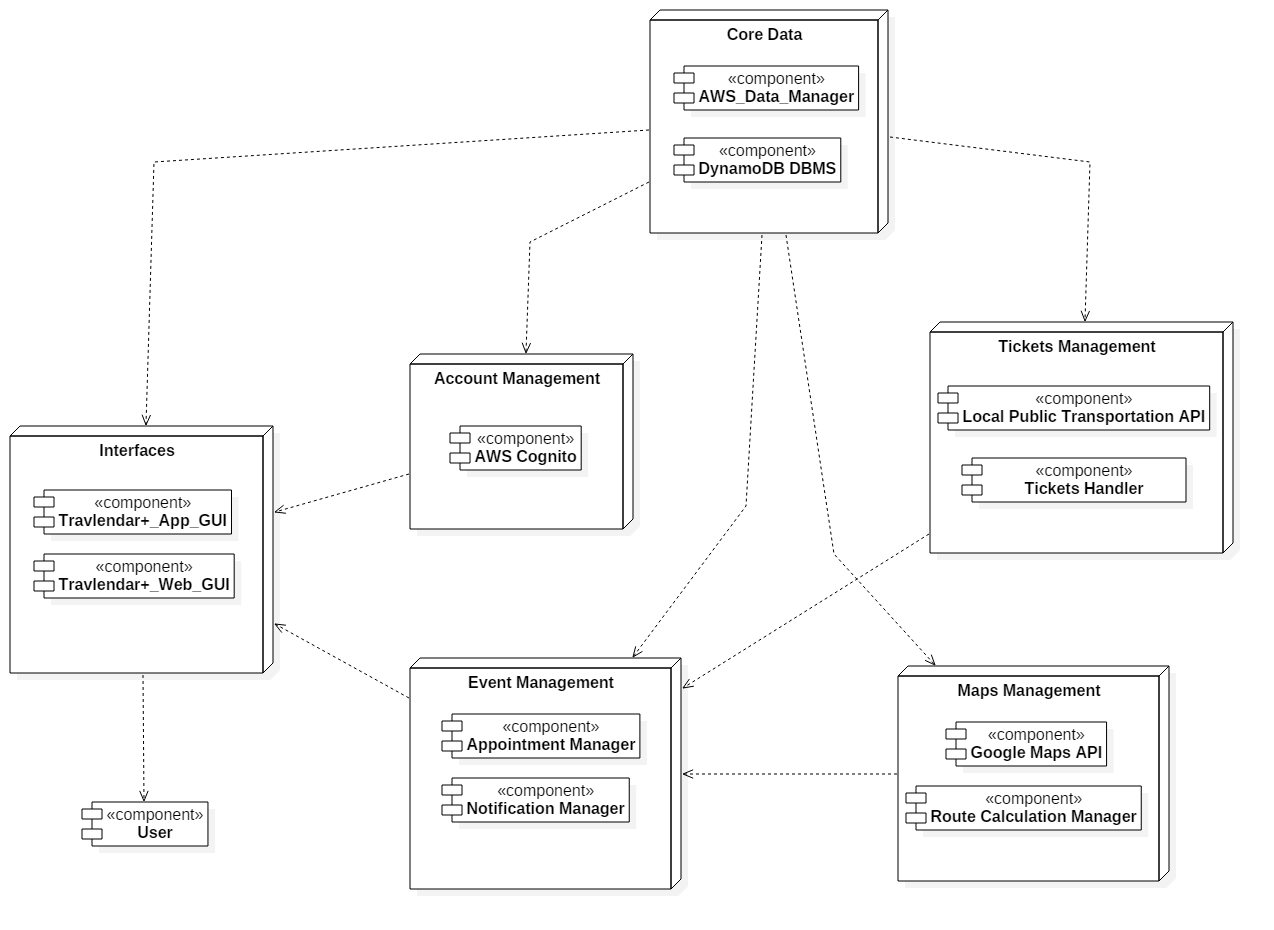
\includegraphics[width=6in]{./diagrams/Integration_Sequence.png}
	\caption{Subsystem Integration Sequence}
	\label{fig:intSequence}
\end{figure}

\vspace*{30px}
\section*{Testing}
We plan to use the following software tools to automate the various tests:
\begin{description}
\item \textbf{xUnit.net}: is a free, open source, community-focused unit testing tool for the .NET Framework. 
We plan to use it for unit test of single components. xUnit features are:
\begin{itemize}
\item Facts are tests that are always true, which test invariant conditions.
\item Theories are tests that are only true for a particular set of data.
\end{itemize}
\item \textbf{Calaba.sh}: Calabash consists of libraries that enable test code to interact programmatically with native and hybrid apps. We use this tools to test the UI of Travlendar+. The interaction consists of a number of end-user actions:
\begin{itemize}
\item Gesture: Touches or gestures, for instance tap, swipe and rotate.
\item Assertion.
\item Screenshots: Screendump the current view on the current device model.
\end{itemize}
\item \textbf{JMater}: is a powerful tool which may be used to test the performance of subsystems, in particular of our web application.
\item \textbf{Xamarin.Profiler}; a great tool that allows us to collect information about our mobile application. We use it to find potential memory leaks, resolve performance bottlenecks, and add polish to the application.
\item \textbf{Browser's debugging}: Since all the main web engines (Google Chrome, Mozilla Firefox, Safari and Microsoft Edge) will be fully supported for the web application, browser's debugging can help too.
\end{description}
If necessary, we might plan to write our own unit tests as well through \textbf{Xamarin.UITest}, which is a testing framework that allows us to automate our UI acceptance testing. 


 

